\documentclass[11pt]{article}

\usepackage[catalan]{babel}
\usepackage{translations}
\usepackage[titles]{tocloft}
\usepackage{multicol}
\usepackage{graphicx} % Required for the inclusion of images
\usepackage{amsmath} % Required for some math elements 
\usepackage{hyperref}
\usepackage{amsmath}
\usepackage{listings}
\usepackage{courier}
\usepackage[margin=1in]{geometry}
\usepackage{changepage}
\usepackage{titlesec}
\usepackage{wrapfig}
\usepackage[version=4]{mhchem}
\usepackage{multirow}
\usepackage{siunitx}
\usepackage{ragged2e}
\usepackage{adjustbox}
\usepackage[font=small,labelfont=bf]{caption}
\usepackage[table,xcdraw]{xcolor}
\usepackage{afterpage}
\usepackage{xfrac}
\usepackage{animate}

\definecolor{codegreen}{rgb}{0,0.6,0}
\definecolor{codegray}{rgb}{0.5,0.5,0.5}
\definecolor{codepurple}{rgb}{0.58,0,0.82}
\definecolor{backcolour}{rgb}{0.95,0.95,0.92}

\lstdefinestyle{mystyle}{
    backgroundcolor=\color{backcolour},   
    commentstyle=\color{codegreen},
    keywordstyle=\color{magenta},
    numberstyle=\tiny\color{codegray},
    stringstyle=\color{codepurple},
    basicstyle=\ttfamily\footnotesize,
    breakatwhitespace=false,         
    captionpos=b,                    
    keepspaces=true,                 
    numbers=left,                    
    numbersep=5pt,                  
    showspaces=false,                
    showstringspaces=false,
    showtabs=false,                  
    tabsize=2
}
\lstset{language=Python, 
        basicstyle=\ttfamily\small, 
        keywordstyle=\color{keywords},
        commentstyle=\color{comments},
        stringstyle=\color{red},
        showstringspaces=false,
        identifierstyle=\color{codepurple},
        keywords=[2]{pow},
        keywordstyle=[2]{\color{orange}},
}

\lstset{style=mystyle}
\setlength\parindent{0pt}
\renewcommand{\labelenumi}{\alph{enumi}.}

\setlength\parindent{0pt} % Removes all indentation from paragraphs

\renewcommand{\labelenumi}{\alph{enumi}.} % Make numbering in the enumerate environment by letter rather than number (e.g. section 6)
   
\newcommand{\titulo}{Determinació de la càrrega\\específica de l'electró\\\ \\(E2)}
\newcommand{\nombreestudiante}{Víctor Mira Ramírez}
\newcommand{\nombredirector}{Ángel Ávila Freire}
\newcommand{\fecha}{\date{Març 2023}}  % Definir solo el año de presentación

\pagebreak

\renewcommand{\listtablename}{Índex de taules} 
\renewcommand{\tablename}{Tabla} 
\renewcommand\cftsecdotsep{\cftdotsep}

\setlength{\cftbeforesecskip}{0.5ex}
\renewcommand{\cftsecfont}{%
  \fontsize{11}{13}\usefont{OT1}{phv}{bc}{n}\selectfont
}
\makeatletter
\renewcommand{\@pnumwidth}{1.75em}
\renewcommand{\@tocrmarg}{2.75em}
\makeatother

\begin{document}

\begin{titlepage}
	\centering
	
\includegraphics[width=65mm]{fotos/logoUA.png}\par
	\vspace{1cm}
	{\huge\bfseries \vspace{15mm} \titulo \par}
	\vfill
	{\large 
	\vfill
	Estudiant:\par\vspace{2mm}
	\nombreestudiante\par
	\vfill
	Professor:\par\vspace{2mm}
    \nombredirector
    \vfill
    Universitat d'Alacant\par
    Facultat de Ciències: Departament de Física Aplicada\par
    Tècniques experimentals I\par
	\fecha\par}
\end{titlepage}

\pagebreak

\begin{abstract}\label{sec:abstract}
    \noindent L'objectiu de la pràctica es descriure la interacció d'electrons accelerats per camps elèctrics i que es troben sota l'acció de camps magnètics. També determinarem la relació càrrega/massa de l'electró gràcies a l'anàlisi anterior.
\end{abstract}

\vspace{0.3cm}
\tableofcontents
\newpage

\section{Introducció i motivació}
    Els objectius de la pràctica son els ja descrits a l'\textit{Abstract}, determinar la relació càrrega-massa de l'electró mitjançant l'estudi del seu comportament quan es troba baix l'efecte d'un camp magnètic després de ser accelerat per una diferència de potencial elèctric. 

    \vspace{0.5cm}Existeixen experiments on la relació càrrega-massa de les partícules és la única magnitud mesurable experimentalment. Amb freqüència, la càrrega de les partícules es pot deduir més fàcilment que la massa, fent que conèixer la relació càrrega-massa ens facilite obtindre la massa de la partícula d'estudi.

    \vspace{0.5cm}A fi de profunditzar en aquests resultats i aportar conclusions, realitzem aquest breu estudi sobre el tema.
    
\section{Marc teòric}
    La física clàssica ens diu que quan una partícula amb càrrega es desplaça per camps electromagnètics, s'apliquen la equació de la Força de Lorentz \ref{eq:lorentz} i la equació de la Segona Llei de Newton \ref{eq:2newton}.
    \begin{equation}
        F = Q\left(E+v\times B\right)
        \label{eq:lorentz}
    \end{equation}
    
    \begin{equation}
        F = ma = m\frac{dv}{dt}
        \label{eq:2newton}
    \end{equation}

    I combinant \ref{eq:lorentz} i \ref{eq:2newton} obtenim:

    \begin{equation}
        \left(\frac{m}{Q}\right)a=E+v\times B
        \label{eq:carregamassa0.5}
    \end{equation}

    on $m$ i $Q$ son la massa i càrrega de la partícula, $E$ i $B$ son els camp elèctric i magnètic i $v$ es la velocitat de la partícula.
    
    \vspace{0.4cm}A la pràctica necessitarem generar un feix d'electrons que utilitzarem com a partícules carregades d'estudi. L'obtindrem per Efecte Termoiònic (veure apèndix \ref{appendix:termoionic}) calfant un filament que actua com a càtode i davant d'ell una placa metàl·lica que actua com a ànode. Aquesta diferència de potencial accelerarà els electrons lliures i generarà el feix d'electrons desitjat.

    \vspace{0.4cm}Per la llei de conservació de l'energia, sabem que l'energia cinètica dels electrons \ref{eq:cinetica} serà igual a l'energia potencial elèctrica proporcionada, i per tant:

    \begin{equation}
        K = U_e =\ \mid e\mid \Delta U
        \label{eq:energies}
    \end{equation}

    \vspace{0.4cm}Considerant que el moviment dels electrons és no-relativista:
    
    \begin{equation}
        K = \frac12 mv^2
        \label{eq:cinetica}
    \end{equation}

    I combinant \ref{eq:energies} i \ref{eq:cinetica} obtenim:

    \begin{equation}
        v = \sqrt{\frac{2\mid e\mid\Delta U}{m}}
        \label{eq:velocitat}
    \end{equation}

    D'altra banda, una vegada coneixem el moviment dels electrons dins de l'emissor, anem a estudiar el seu comportament una vegada es veuen afectats per el camp magnètic de les bobines. Coneixem la Llei de Lorentz \ref{eq:lorentz}, que ens diu que una partícula carregada en moviment dins d'un camp magnètic es vorà afectada per una força perpendicular al pla que formen $\overline{v}$ i $\overline{B}$. Per tant un feix de partícules carregades que segueixen una trajectòria lineal com el que tenim, es vorà afectat per una força magnètica de forma que traçarà una nova trajectòria,una òrbita circular. En mòdul la força magnètica:

    \begin{equation}
        F_B = \mid e\mid v B
        \label{eq:fb mod}
    \end{equation}

    \vspace{0.4cm}Com sabem que l'electró es una partícula amb massa, sabem que experimentarà una força centrípeta $F_c$ igual a la força magnètica $F_B$.

    \begin{equation}
        F_c = m\frac{v^2}{r}
        \label{eq:fc}
    \end{equation}

    I combinant \ref{eq:fb mod} i \ref{eq:fc} obtenim:

    \begin{equation}
        F_B = F_c \Longleftrightarrow\  \mid e\mid v B = m\frac{v^2}{r}
        \label{eq:fb}
    \end{equation}

    A més, com coneixem la velocitat que portarà per \ref{eq:velocitat}, podem introduir-la a l'última equació i obtindre:

    \begin{equation}
        \frac{\mid e\mid}{m}=\frac{2\Delta U}{B^2r^2}
        \label{eq:carregamassa0.9}
    \end{equation}

    \vspace{0.4cm}Per acabar, hem de conèixer una expressió per al camp magnètic generat per les bobines, a fi de simplificar \ref{eq:carregamassa0.9}. La densitat de flux magnètic $B$ en el punt mitjà entre les bobines s'expressa:

    \begin{equation}
        B = \left(\frac45\right)^{\sfrac{3}{2}}\frac{\mu_0nI}{R}
        \label{eq:bhelmholtz}
    \end{equation}

    \vspace{0.4cm}Finalment, combinem \ref{eq:carregamassa0.9} i \ref{eq:bhelmholtz} per a obtindre una expressió per a la relació càrrega massa de l'electró al nostre experiment i obtenim:

    \begin{equation}
        \boxed{
            \frac{\mid e\mid}{m}=\left(\frac{5}{4}\right)^3\frac{2R^2\Delta U}{\mu_0^2 N^2 r^2 I^2}
        }
        \label{eq:carregamassa}
    \end{equation}

    \vspace{0.2cm}on $R$ i $N$ son el radi i el nombre d'espires de les bobines de Helmholtz, $I$ és la intensitat que circula per les bobines, $\mu_0$ es la permeabilitat magnètica del buit i $r$ i $\Delta U$ son el radi del feix d'electrons i la diferència de potencial aplicada a l'emissor.
    
\clearpage
\section{Procediment experimental}
    \subsection{Material}
        \begin{multicols}{2}
            \begin{itemize}
                \item Cables.
                \item Dos multímetres.
                \item Bobines de Helmholtz (veure apèndix \ref{appendix:helmholtz}).
                \item Esfera de vidre a baixa pressió ($0.1\si{\pascal}$).
                \item Font d'alimentació alterna de $6.3\si{\volt}$ (emissor).
                \item Font d'alimentació continua de $300\si{\volt}$ (bobines).      
                \item Tub de raigs catòdics.
                \item Canó d'electrons.
                      \begin{itemize}
                          \item Filament emissor.
                          \item Placa metàl·lica.
                          \item Reixeta reguladora.
                      \end{itemize}
            \end{itemize}
        \end{multicols}

        Les nostres bobines constaven de $154$ espires cadascuna ($14$ capes amb $11$ espires per capa), la resistència de cada bobina és de $2.1\si{\ohm}$ i el corrent màxim que poden suportar és de $3\si{\ampere}$.

        \vspace{0.4cm}Després de realitzar tres mesures del diàmetre de les bobines en punts diferents: 0.416, 0.416 i 0.417 $\pm$ 0.001 metres, obtenim (després del tractament estadístic i de l'error) un valor per al radi de: $R = (0.208 \pm 0.002)\si{\meter}$
        
    \subsection{Metodologia} 
        \begin{wrapfigure}[9]{l}{.22\textwidth}
            \label{fig:disposicio}
            \vspace{-0.9cm}
            \begin{center}
                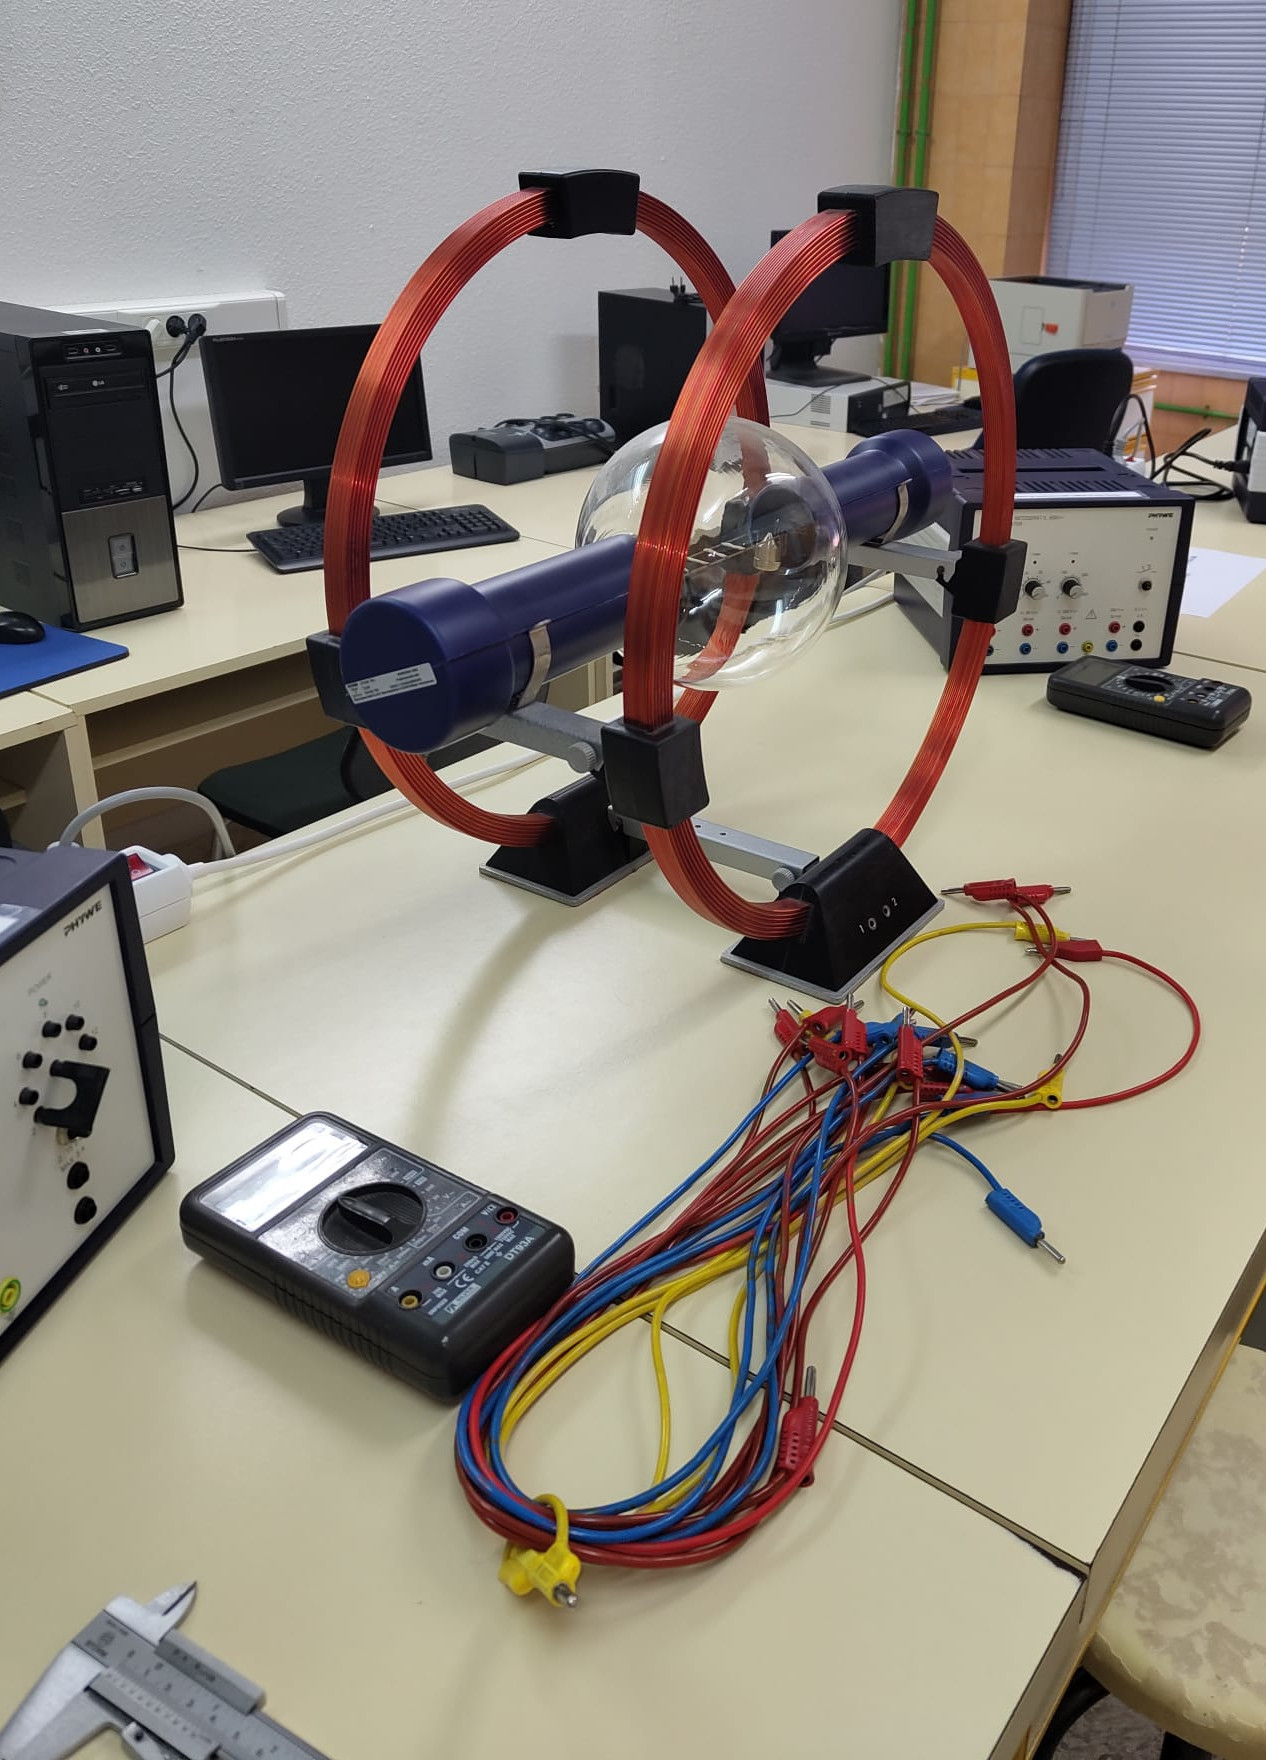
\includegraphics[width=.2\textwidth]{fotos/disposicion.jpeg}
            \end{center}
        \end{wrapfigure}
        L’experiment realitzat en el laboratori va consistir d'un recinte esfèric tancat (amb un gas a pressió de $0.1\si{\pascal}$). Dins de l'esfera trobem un tub de raig catòdics i un emissor d'electrons. Quan connectem l'emissor a la font d'alimentació de corrent continua, aquest comença a emetre electrons, que segueixen una trajectòria lineal.
        
        \vspace{0.4cm}Per l'acció del camp magnètic generat per les dos bobines de Helmholtz connectades a la font d'alimentació de corrent continua, els electrons canviaran la seua trajectòria lineal per una circular, i col·lisionaràn amb el tub de raig catòdics, emetent llum.

        \vspace{0.4cm}A la figura anterior \ref{fig:disposicio}, trobem la disposició experimental. Observem les dues fonts d'alimentació, els multímetres i cables, i finalment les bobines i l'esfera amb els tubs de raigs catòdics i l'emissor d'electrons.

        \vspace{0.4cm}Com sabem, el feix d'electrons produït tindrà una trajectòria circular gracies al camp magnètic de les bobines de Helmholtz. El radi d'aquesta trajectòria dependrà de la intensitat del camp magnètic a més de la velocitat dels electrons del feix. Es a dir, en funció del voltatge aportat a les bobines i a l'emissor obtindrem trajectòries de diversos radis.

        \vspace{0.4cm}Experimentalment, fixem el voltatge de l'emissor i variem el de les bobines. D'aquesta manera anotem la intensitat i voltatge necessaris per a arribar a quatre radis: $5,4,3\text{ i }2$cm. Les dades obtingudes es troben a l'apèndix \ref{appendix:dades}.

\clearpage
\section{Resultats i discussió}
    \vspace{0.2cm}Amb les dades obtingudes i l'equació \ref{eq:carregamassa}, tractem d'obtindre un valor per a la relació càrrega massa de l'electró. Per a fer-ho, grafiquem l'expressió equivalent: (amb forma $y=mx + b$)

    \begin{equation}
        \left(\frac{5}{4}\right)^3\frac{2R^2}{\mu_0^2 N^2}\ \frac{\Delta U}{r^2} = \frac{\mid e\mid}{m}\ I^2
        \label{eq:carregamassaLineal}
    \end{equation}

    on $y$ es un nombre conegut que anomenarem $S$ i multiplica a $\frac{\Delta U}{r^2}$, $x$ és $I^2$ i la pendent $m$ es la relació càrrega massa que volem calcular.

    \[S=\left(\frac{5}{4}\right)^3\frac{2R^2}{\mu_0^2 N^2}\]

    \vspace{0.4cm}Per a cada radi tindrem una gràfica i valors per a la pendent distints com observem a la figura següent:

    \begin{figure}[h]
        \centering
        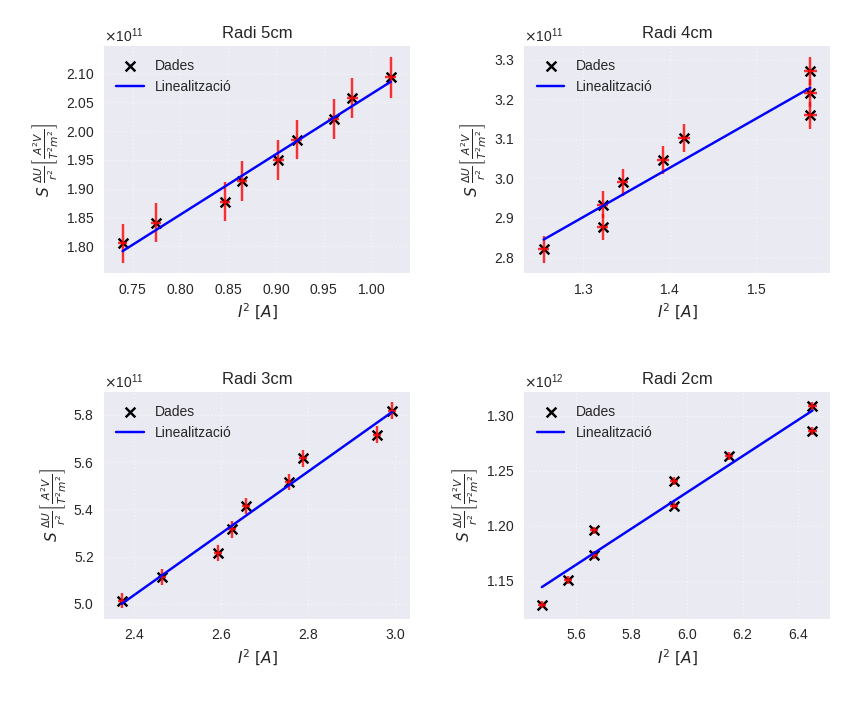
\includegraphics[width=0.85\textwidth]{fotos/4graphs.png}
        \caption{Linealització per a diferents radis}
        \label{fig:4graph}
    \end{figure}

    Observem com les barres d'error no s'acomoden a les linealitzacions ja que estem enfocant el càlcul d'una manera massa aïllada, els valors obtinguts a cada tabla per a la pendent s'allunyen més del 80\% del valor de la literatura.
    
    \clearpage
    Per això, el més fiable es graficar tots els radis a una mateixa gràfica, ja que la relació càrrega massa es manté constant independentment del radi de la trajectòria. De la pendent de la gràfica \ref{fig:1graph} obtenim el valor de la relació que estàvem esperant.

    \vspace{-0.5cm}
    \begin{figure}[h]
        \centering
        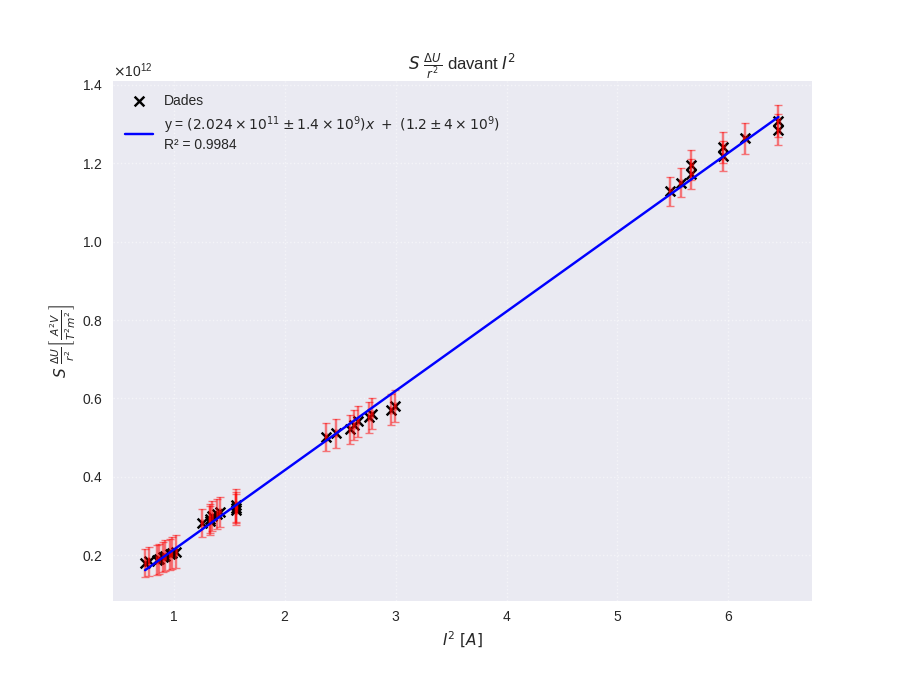
\includegraphics[width=0.78\textwidth]{fotos/1graph.png}
        \caption{Linealització de l'equació \ref{eq:carregamassaLineal}}
        \label{fig:1graph}
    \end{figure}

    La pendent té un valor de $2.024\times10^{11} \pm 1.4\times10^9\si{\coulomb}/\si{\kilogram}$, un poc major al de la literatura, $1.77\times10^{11}\si{\coulomb}/\si{\kilogram}$. L'error relatiu seria del $14\%$. El càlcul dels errors es troba detallat a l'apèndix \ref{appendix:error}.
    \subsection{Camp magnètic desalineat}
        Una qüestió curiosa és observar el que passa quan girem les bobines de Helmholtz respecte de l'eix en que els electrons son emesos.

        \begin{figure}[h]
            \begin{center}
                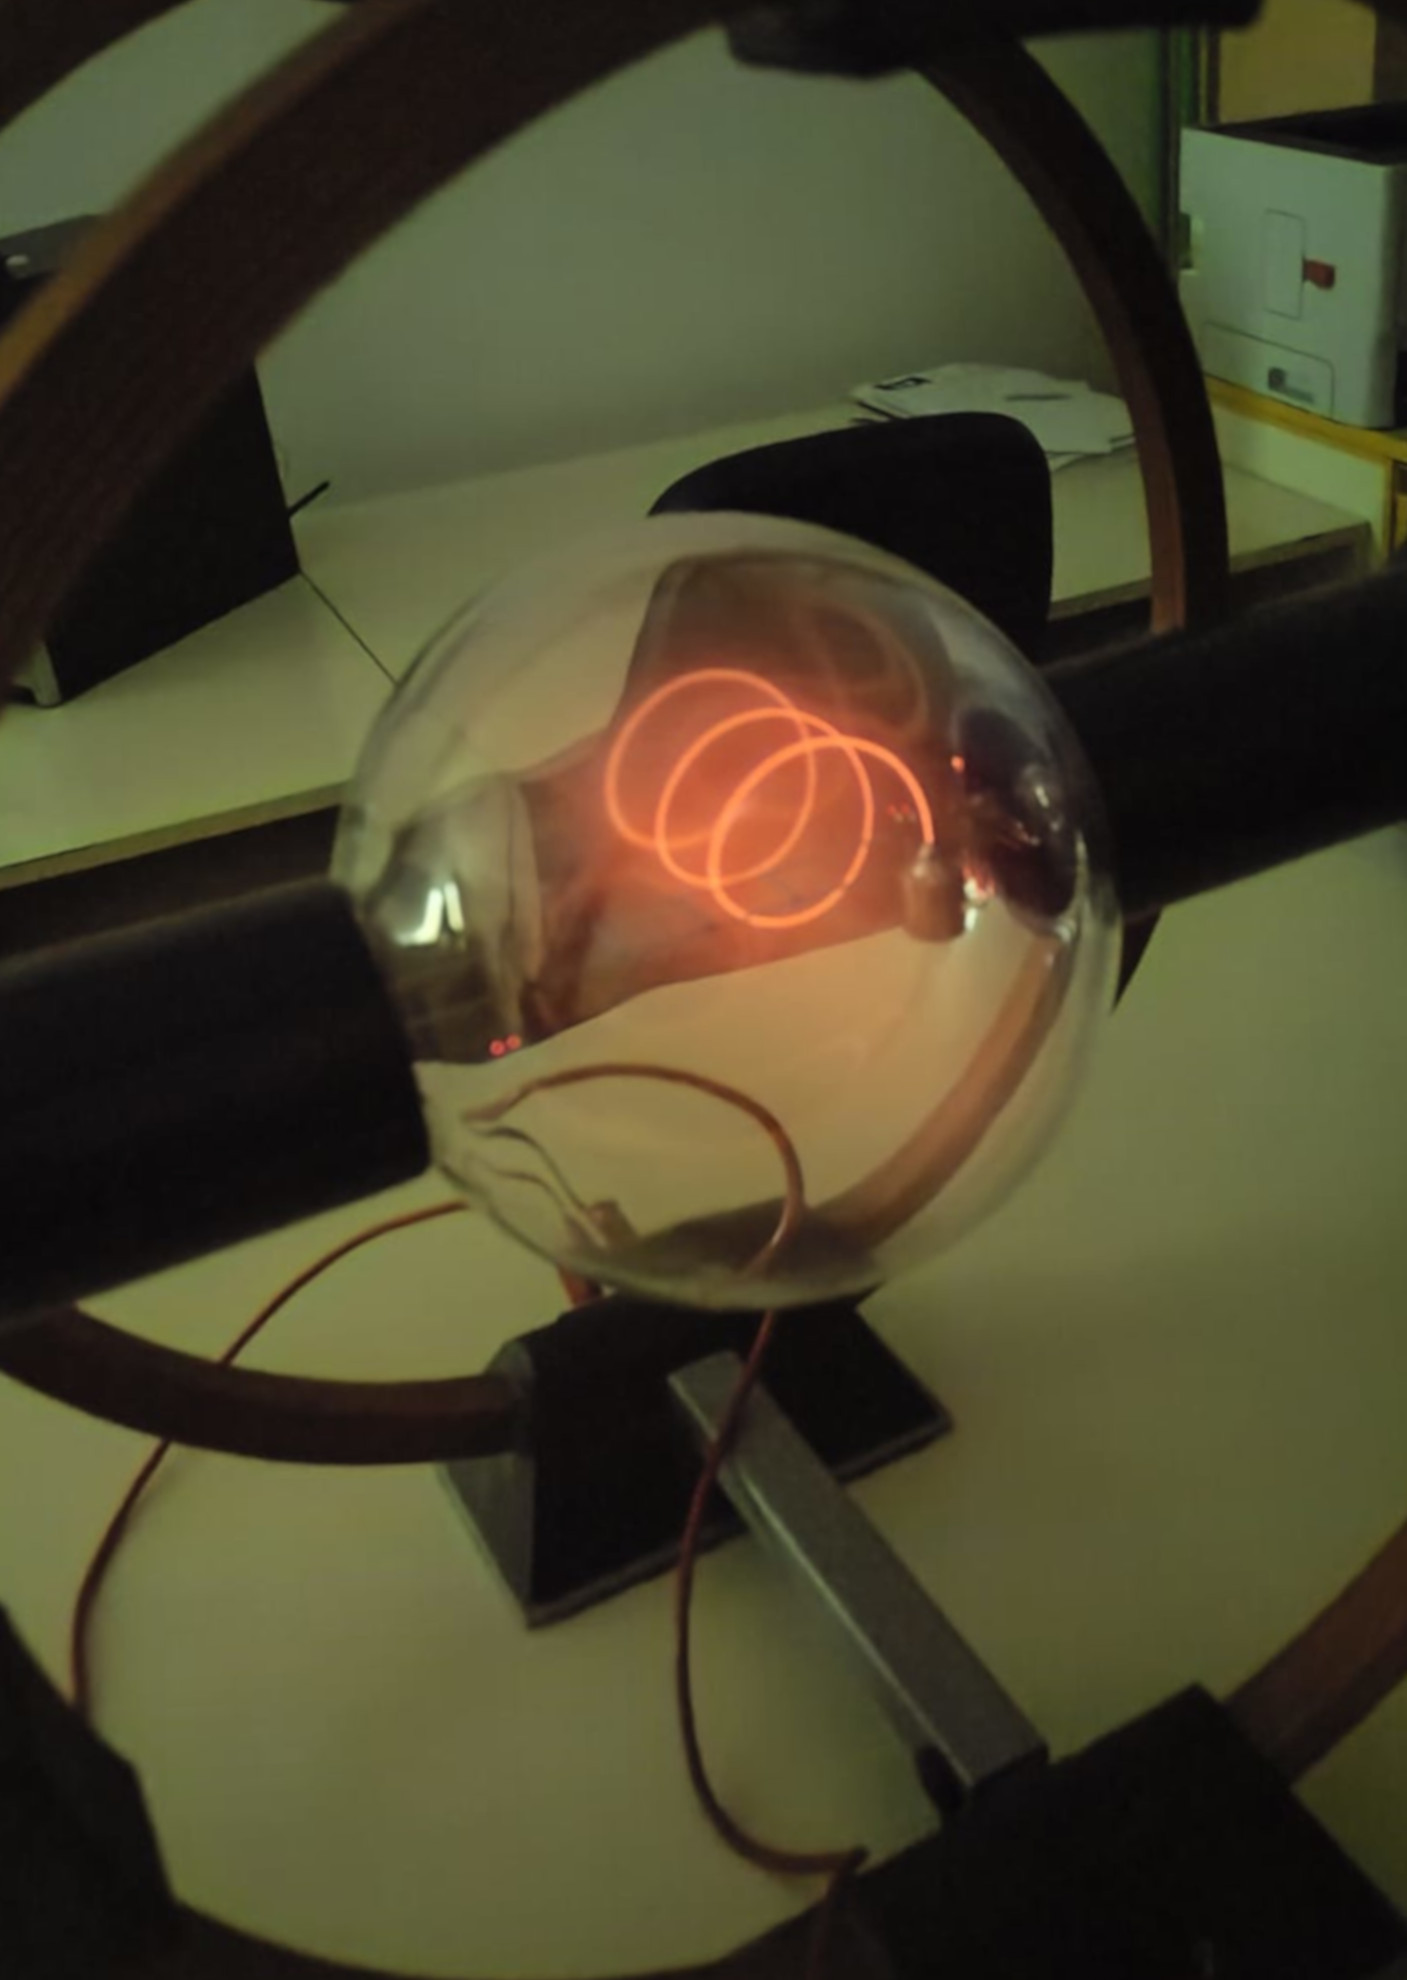
\includegraphics[width=.2\textwidth]{fotos/gif/espiral1.jpeg}
                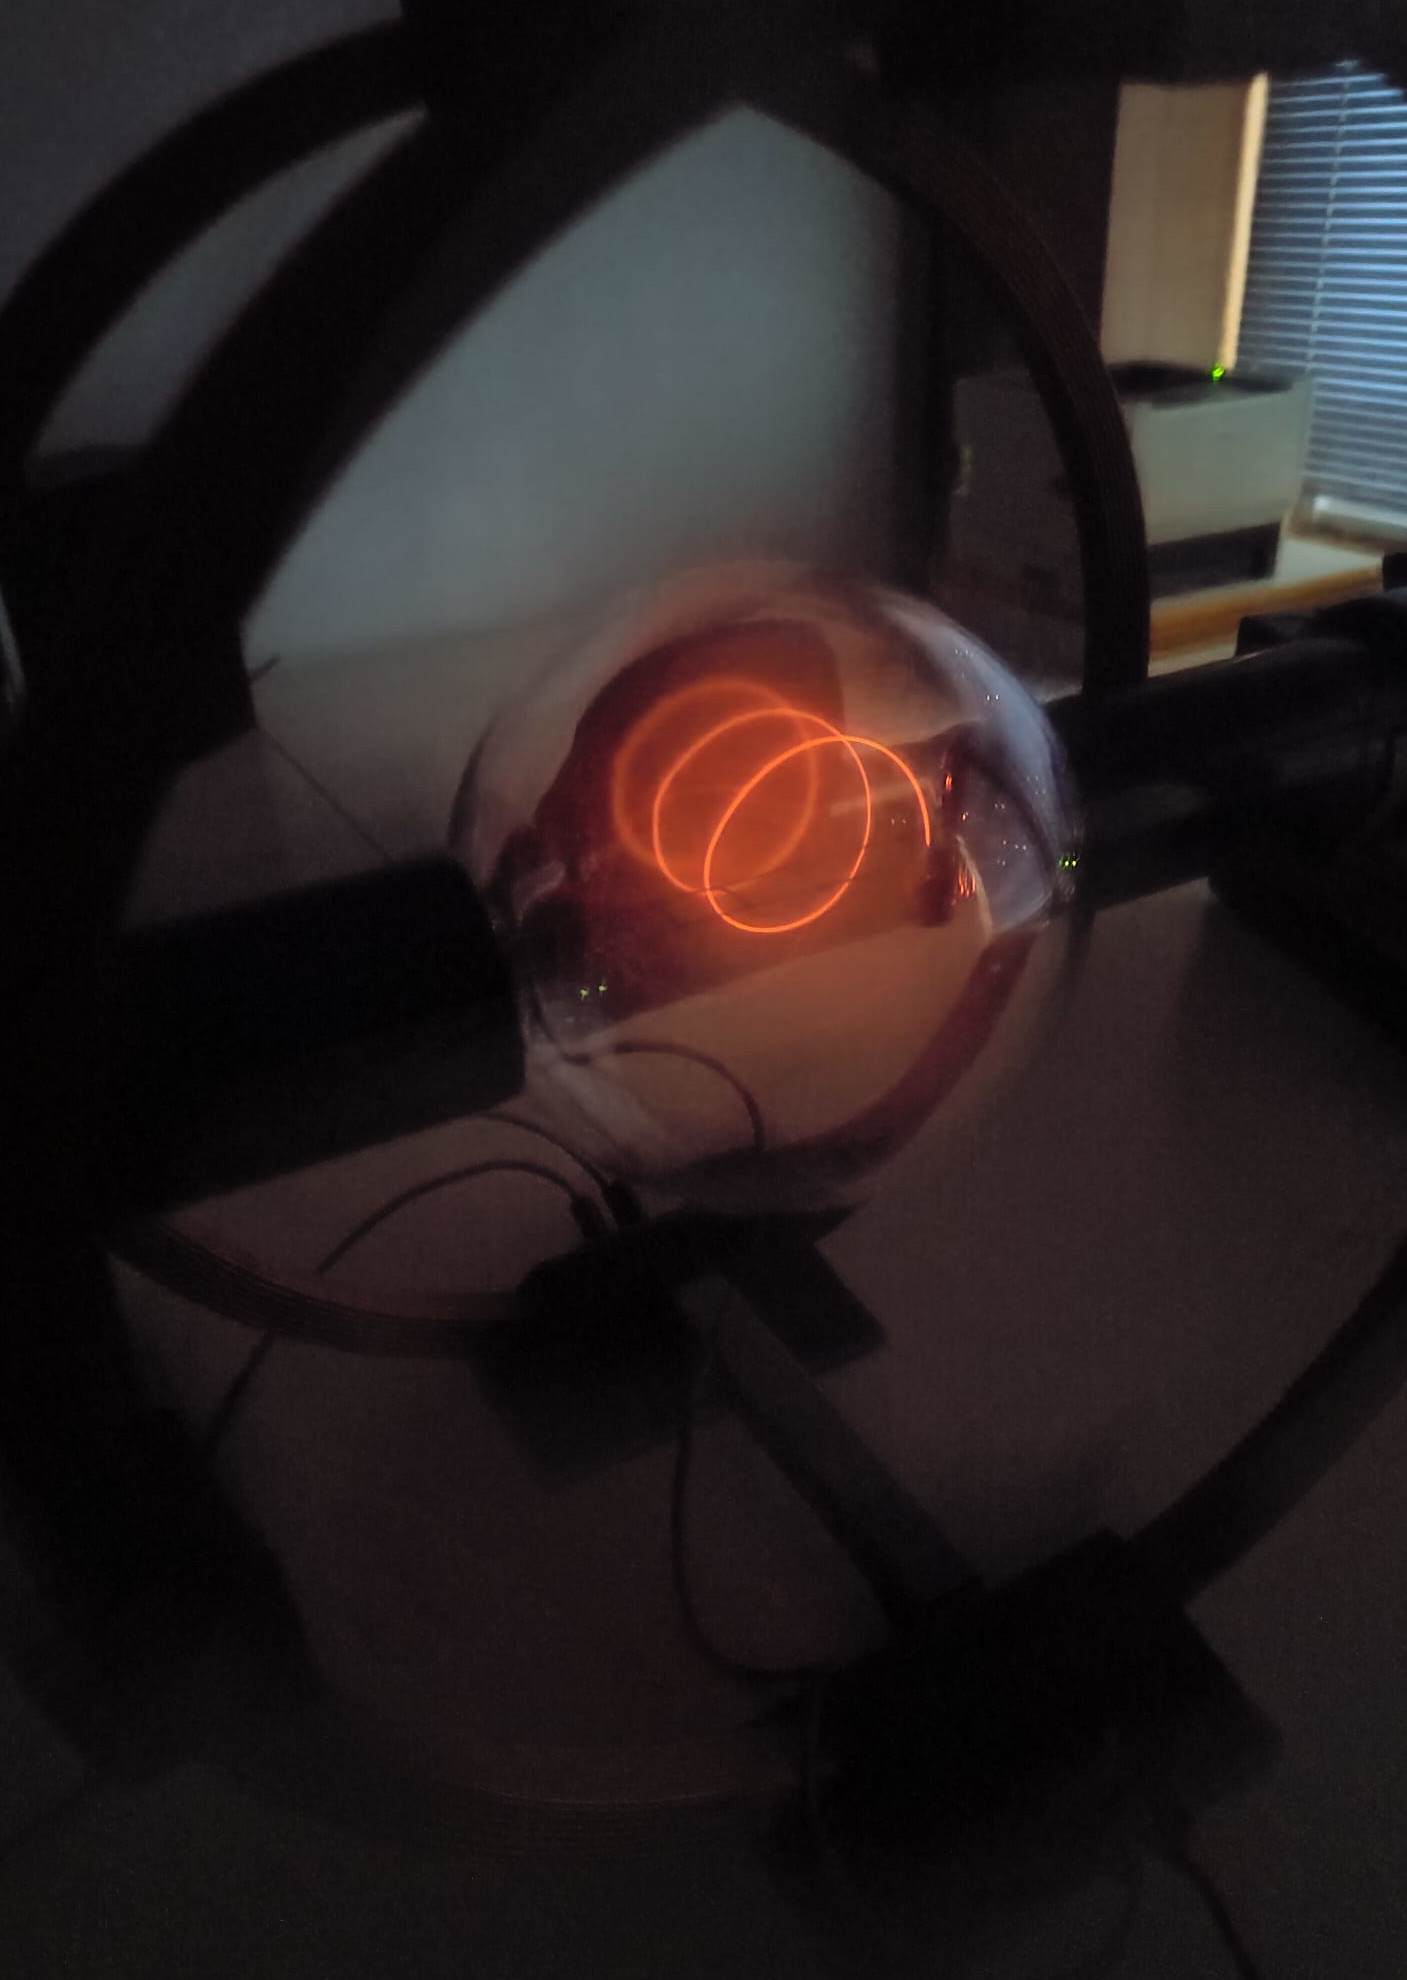
\includegraphics[width=.2\textwidth]{fotos/gif/espiral2.jpeg}
                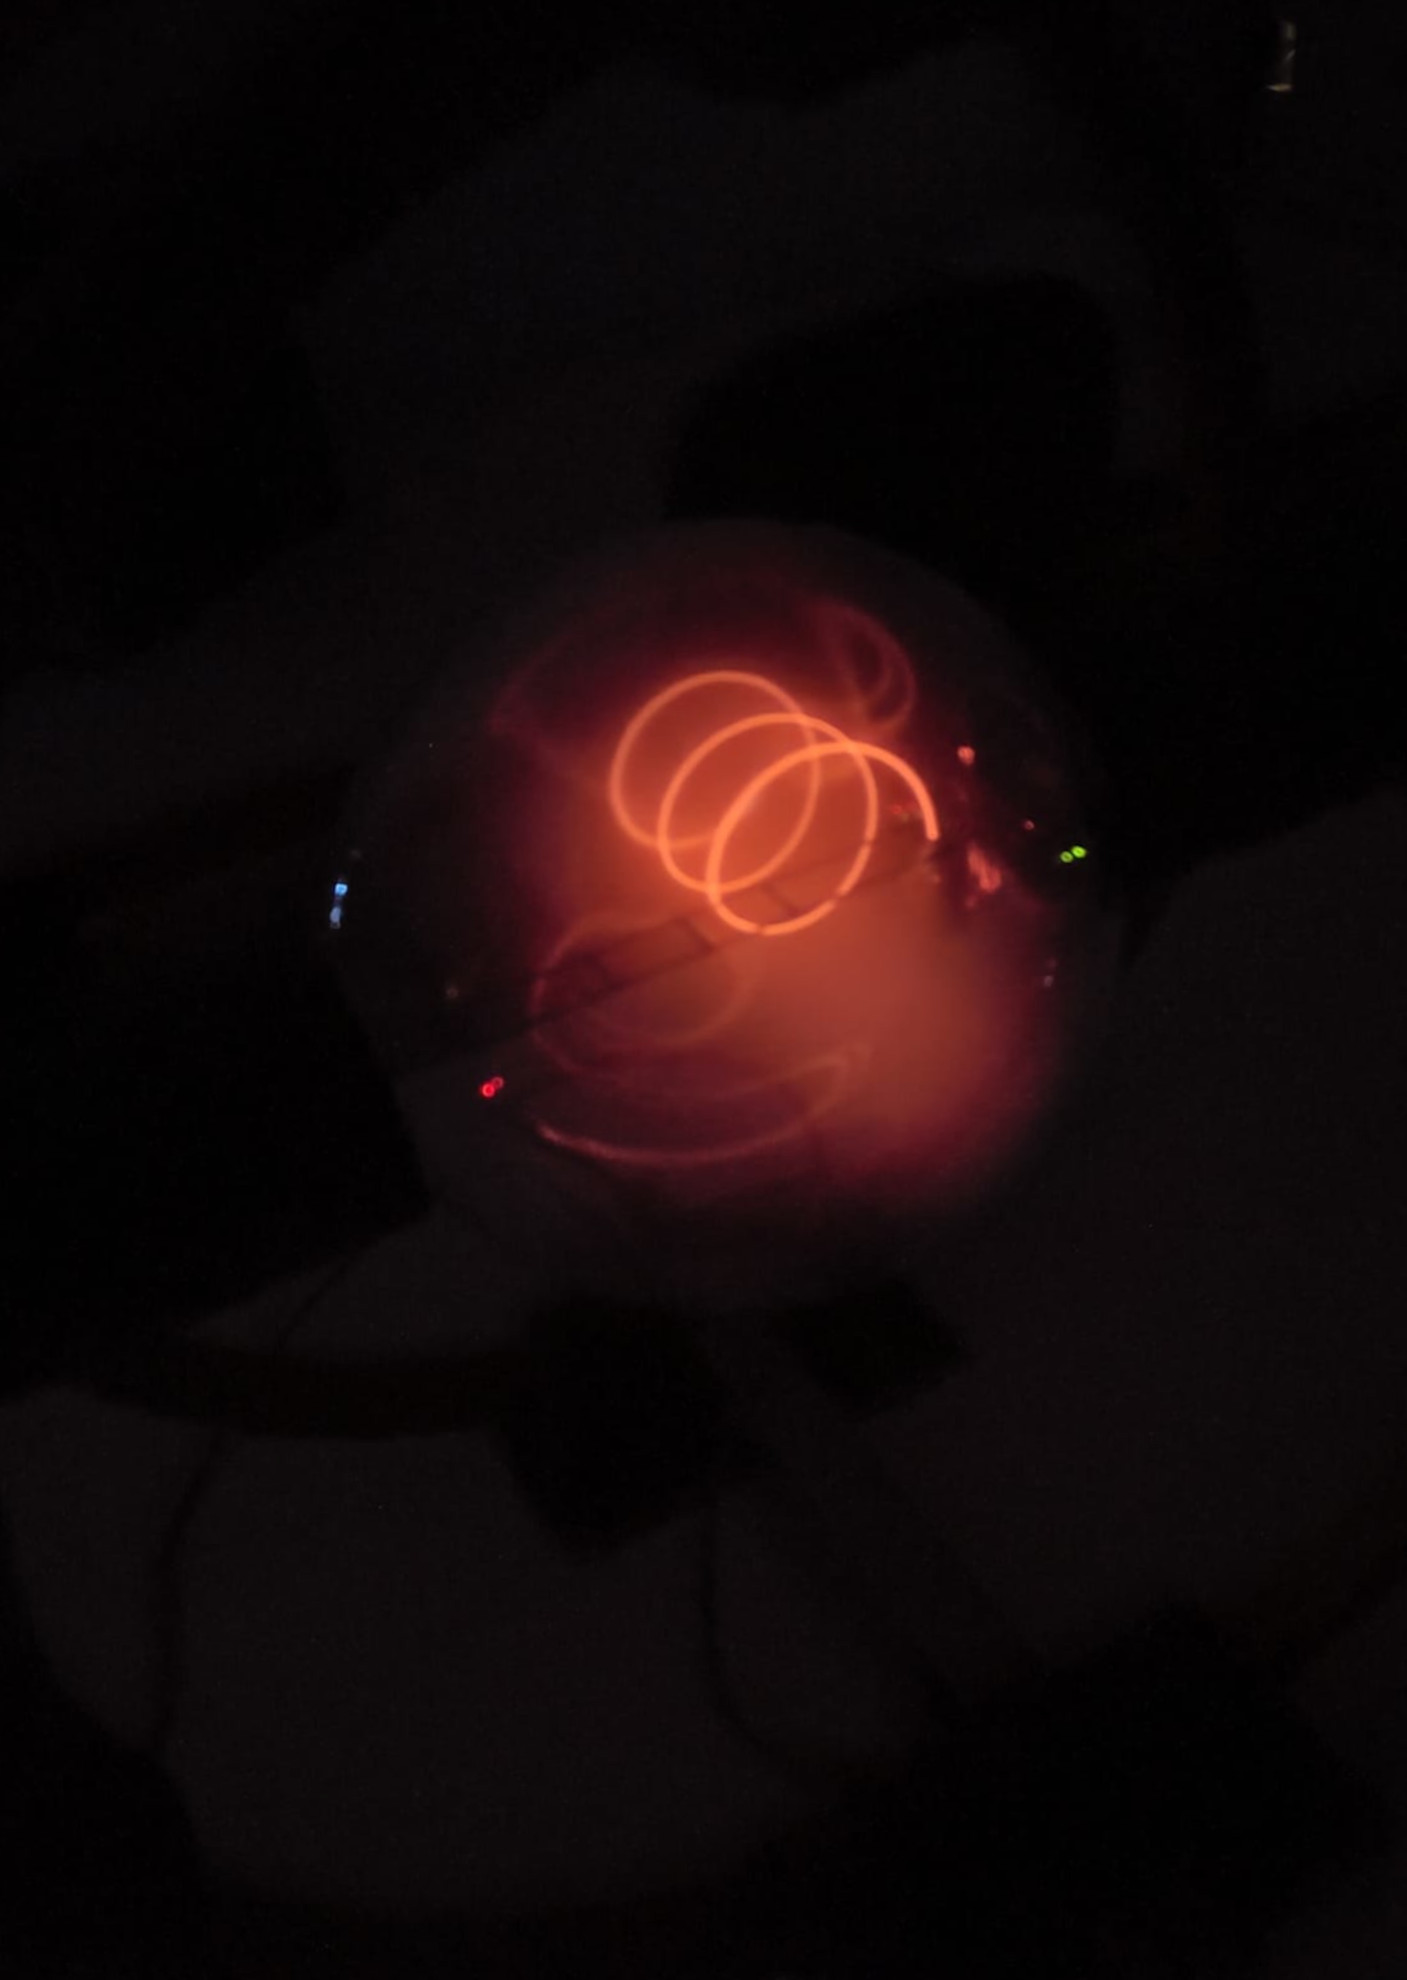
\includegraphics[width=.2\textwidth]{fotos/gif/espiral3.jpeg}
            \end{center}
        \end{figure}

        Aquestes vistoses imatges son el producte de un angle que no siga perfectament perpendicular entre el feix i les línies de camp magnètic, el que fa que el feix tinga un desplaçament en altra direcció espacial.
\section{Possibilitats de millora}
    Tot i que l'error relatiu obtingut es acceptable, anem a discutir algunes possibles fonts d'error i suggerències de millora. Estaria bé estudiar si l'efecte relativista és o no un factor important a l'hora de fer esta pràctica, encara que siga negligible, la teoria de la relativitat es un camp d'estudi al qual els alumnes d'aquesta assignatura profunditzen al quatrimestre anterior i personalment considere que seria una bona aportació al material de la pràctica. 

    \vspace{0.4cm}En el que fa a la realització de la pràctica, probablement haguérem obtingut un valor per a la relació càrrega massa més proper al de la literatura si haguérem utilitzat un rang de voltatges més ample al que vam utilitzar (100 - 116)V. Aquesta observació queda clara quan presentem la figura \ref{fig:1graph}, i les dades son molt denses al voltant d'una intensitat concreta, però entre dades n'hi ha salts prominents.

    \vspace{0.4cm}També recalcar la importància de mesurar correctament el diàmetre de les bobines, que fluctuant mínimament canvien de forma dràstica el valor obtingut. Determinar quan el feix feia que els tubs de raigs catòdics s'iluminaven plenament no era rigorós del tot i òbviament va ser altra font d'error humà. 
\section{Conclusions}
    \begin{wrapfigure}{l}{.253\textwidth}
        \vspace{-0.89cm}
        \begin{center}
            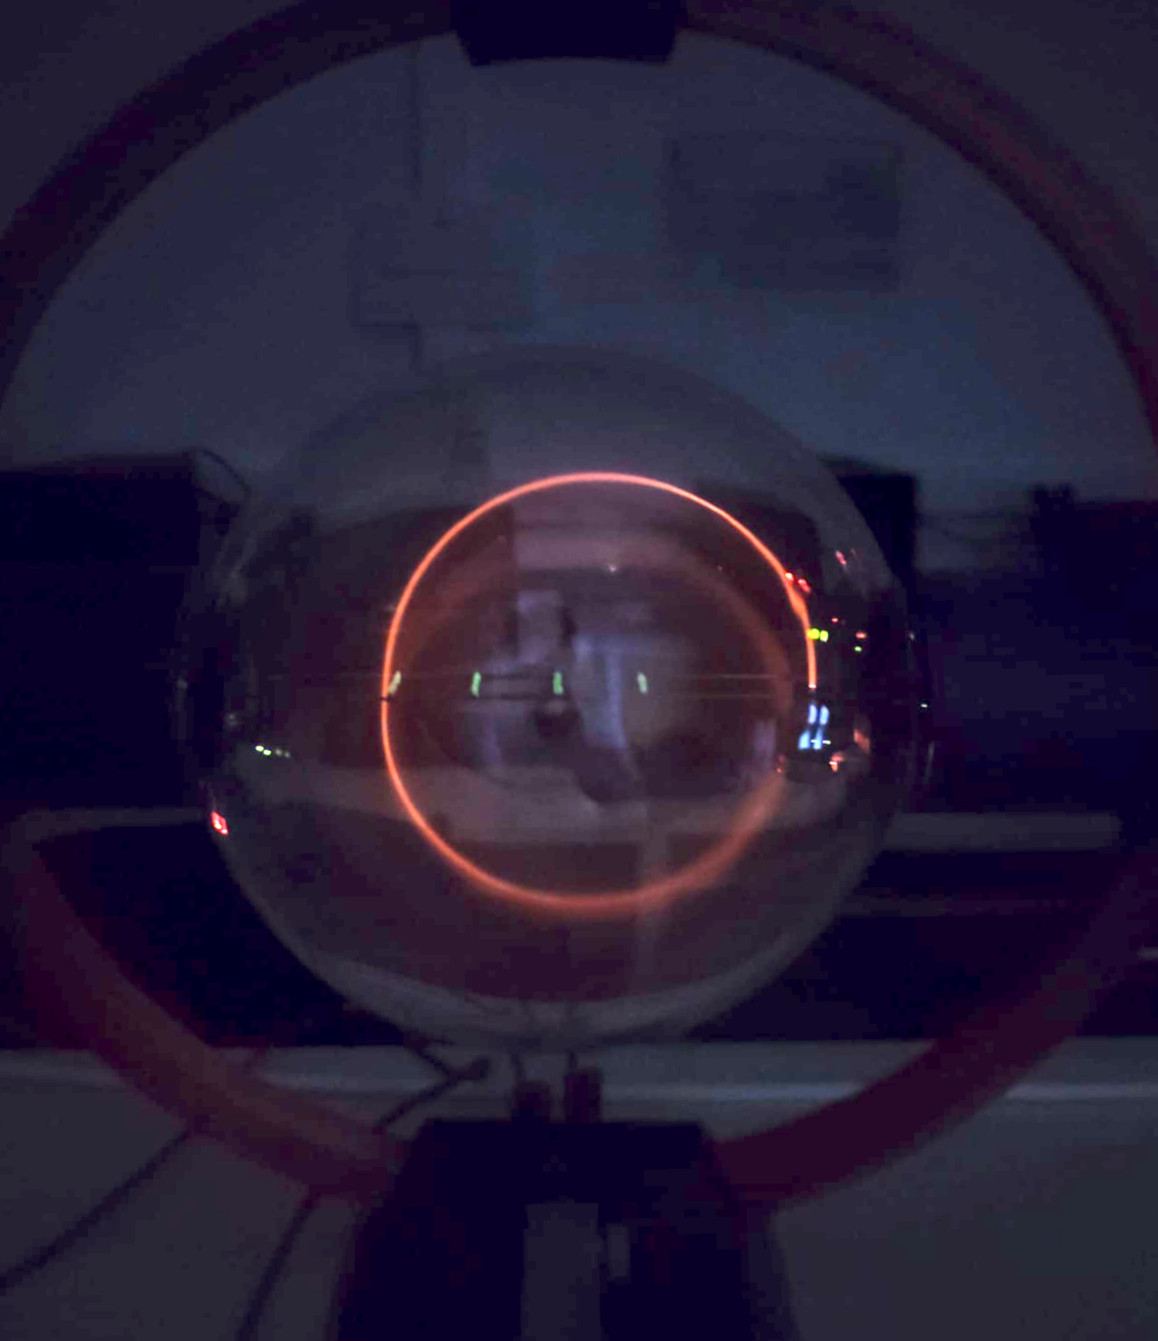
\includegraphics[width=.253\textwidth]{fotos/feix.jpeg}
        \end{center}
    \end{wrapfigure}
    A aquest informe es detalla el càlcul de la relació càrrega massa de l'electró mitjançant l'estudi del seu moviment dins d'un camp magnètic. 
    
    \vspace{0.35cm}La suposició d'un moviment no-relativista juntament amb un error de plantejament a l'hora de fer les mesures experimentals han introduït unes imprecisions considerables que caldria resoldre amb una nova toma de mesures més adequades.

    \vspace{0.35cm}La figura mostra l'experiment en funcionament, tot i que la exposició de la imatge ha sigut modificada a posteriori per a facilitar la seua visualització (l'experiment es va realitzar a una foscor plena).

\clearpage
\section{Apèndixs}
    \vspace{0.4cm}
    \subsection{Bobina de Helmholtz}\label{appendix:helmholtz}
        \vspace{0.2cm}
        \begin{wrapfigure}{l}{.25\textwidth}
            \vspace{-0.89cm}
            \begin{center}
                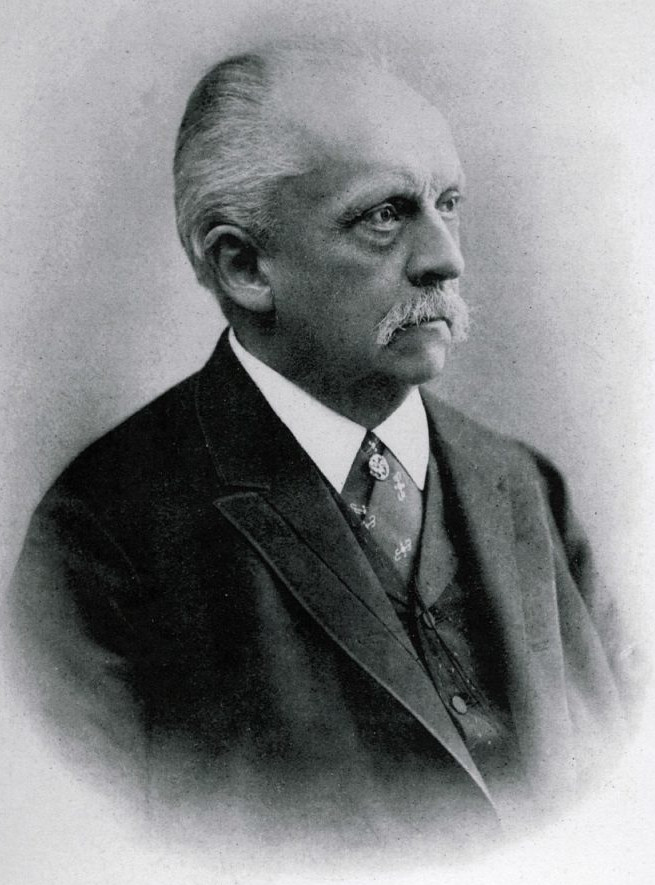
\includegraphics[width=.245\textwidth]{fotos/helmholtz.jpeg}
            \end{center}
        \end{wrapfigure}
        Una Bobina de Helmholtz és un dispositiu per a crear un camp magnètic quasi uniforme en una regió concreta de l'espai. Porta el nom del físic i mèdic \textit{Hermann Ludwig Ferdinand von Helmholtz}. Destaquen les seues contribucions a la electrodinàmica i termodinàmica, així com els seus treballs en fisiologia i psicologia centrats a l'estudi de la percepció visual i auditiva humana. Es conegut per la seua filosofia de la ciència, orientada també a la percepció humana i les lleis naturals.
        
        \vspace{0.4cm}El formen dos solenoides situats a un mateix eix espacial. A més de crear camps magnètics, les bobines de Helmholtz també s'utilitzen en aparells científics per cancel·lar els camps magnètics externs, com ara el camp magnètic de la Terra.
        
        \vspace{0.5cm}\hspace{-0cm}Un parell de bobines de Helmholtz consisteix en dues bobines magnètiques circulars idèntiques (solenoides) que es col·loquen simètricament al llarg d'un eix comú, una a cada costat de l'àrea experimental, i separades per una distància $h$ igual al radi $R$ de la bobina. A cada bobina hi circula un corrent elèctric de la mateixa intensitat i en el mateix sentit.

        \begin{wrapfigure}{r}{.3\textwidth}
            \vspace{-0.9cm}
            \begin{center}
                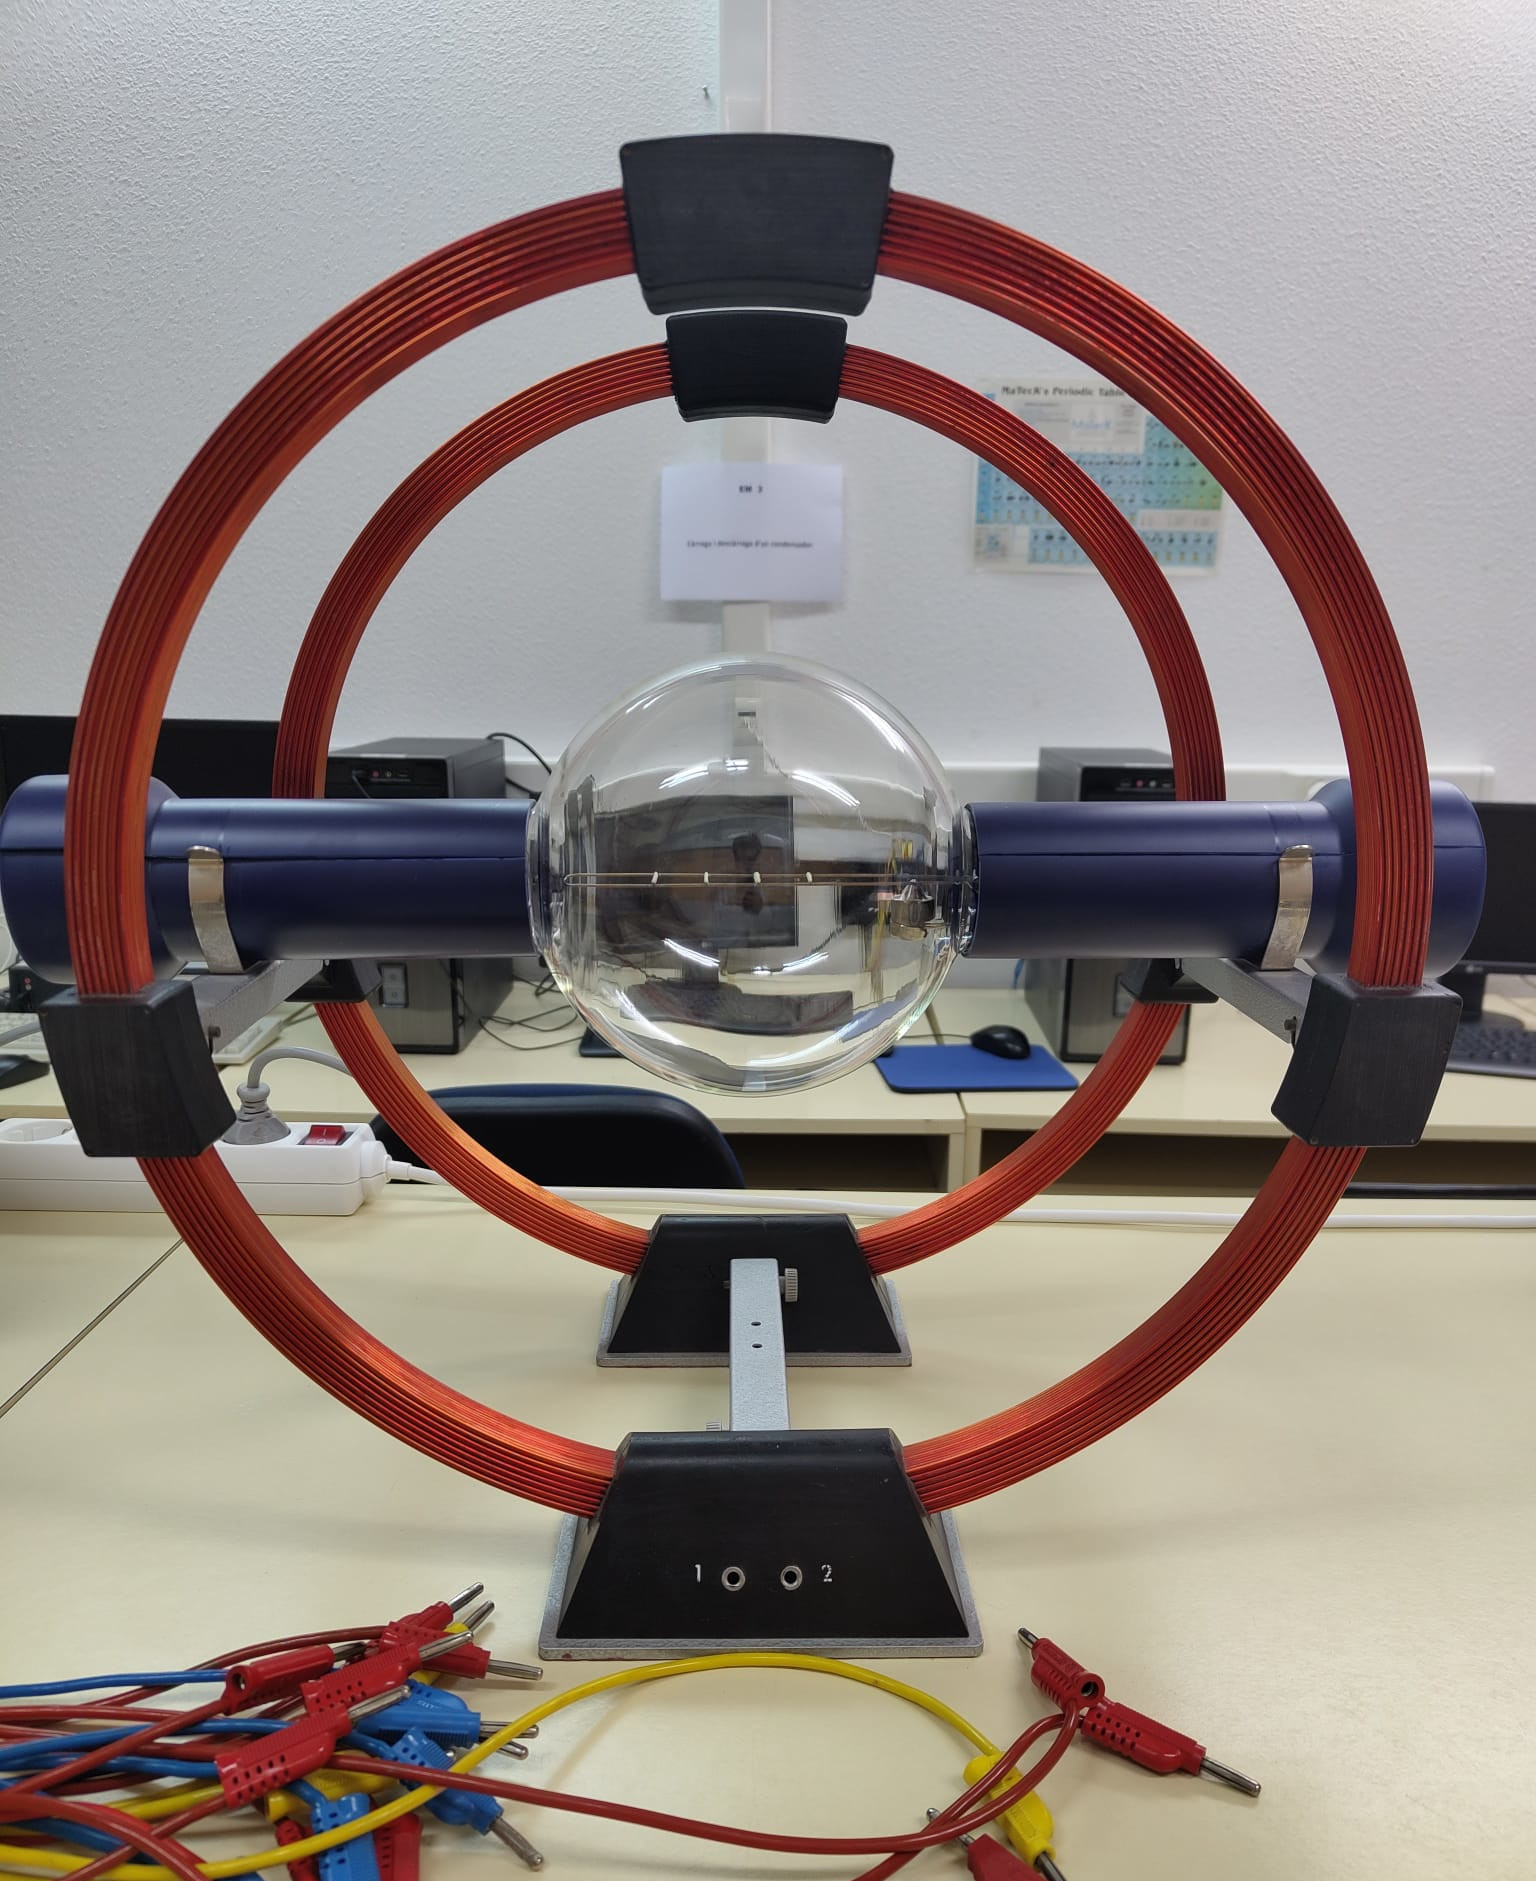
\includegraphics[width=.3\textwidth]{fotos/bobina.jpeg}
            \end{center}
        \end{wrapfigure}

        
        \vspace{0.4cm}Per millorar la uniformitat del camp a l'espai dins de les bobines, es poden afegir unes bobines addicionals a l'exterior. James Clerk Maxwell va mostrar el 1873 que una tercera bobina de major diàmetre situada entre les dues bobines de Helmholtz podia reduir considerablament les variacions del camp magnètic. Aquesta disposició especial s'anomena Bobina de Maxwell.

        \vspace{0.4cm}El càlcul exàcte del camp magnètic en qualsevol punt de l'espai és matemàticament complex i implica l'estudi de la funció de Bessel. La situació és més simple al llarg de l'eix del parell de bobines: és convenient fer del desenvolupament en sèrie de Taylor de la intensitat de camp en funció de $x$, la distància des del punt central de les bobines al llarg de l'eix. 

        \vspace{0.5cm}\hspace{-0cm}El càlcul que es detalla a continuació dona el valor exacte del camp magnètic en el punt central. Si el radi és R, el nombre de voltes a cada bobina és n i el corrent a través de les bobines és I, llavors la densitat de flux magnètic B en el punt mitjà entre les bobines vindrà donada per:
        \[B = \left(\frac45\right)^{\sfrac{3}{2}}\frac{\mu_0nI}{R}\]
        \clearpage
    \subsection{Raigs X}
        \begin{wrapfigure}[5]{r}{.33\textwidth}
            \vspace{-0.9cm}
            \begin{center}
                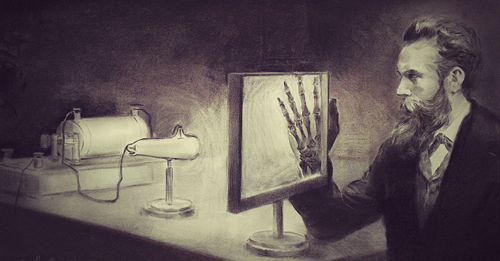
\includegraphics[width=.31\textwidth]{fotos/rayosx.jpg}
            \end{center}
        \end{wrapfigure}
        
        Els termes raigs X i radiació X designen una part de l'espectre electromagnètic que correspon a radiació menys energètica que els raigs gamma i més que els raigs ultraviolats. La longitud d'ona d'aquestes radiacions ionitzants està compresa entre deu nanòmetres i cent picòmetres.

        \vspace{0.5cm}Foren descoberts pel físic alemany \textit{Wilhelm Röntgen} el 1895, que va ser qui els va donar el nom de "raigs X". A alguns països com Alemanya, aquests raigs s'anomenen raigs Röntgen en el seu honor.

        \vspace{0.4cm}El mètode bàsic de generar artificialment raigs X és mitjançant una acceleració d'electrons per fer-los xocar amb un metall. Dins del material els electrons es veuen sobtadament frenats i, amb la gran quantitat d'energia que porten, poden extraure electrons dels nivells més interns dels àtoms del metall.

        \vspace{0.4cm}Com a resultat, un electró dels nivells superiors "cau" a un nivell inferior per omplir el buit i en el procés emet energia en forma de fotó, que anomenarem fotó de raigs X. Actualment també es poden generar raigs X en els sincrotrons.

        \vspace{0.4cm}La disponibilitat d'aquesta font controlable de raig X va crear el camp de radiografia, la imatge d'objectes opacs a la radiació electromagnètica (llum) amb radiació penetrant. A diferència d'altres fonts de radiació ionitzant, només es produeixen radiografies mentre el tub de raigs X està actiu. Els tubs de raigs X també s'utilitzen en els escàners d'equipatges de l'aeroport, anàlisi de materials i estructures i per a la inspecció industrial i en general qualsevol aplicació que requerisca vore a través de materials opacs relativament prims.

        \vspace{0.4cm}
        \begin{figure}[h]
            \centering
            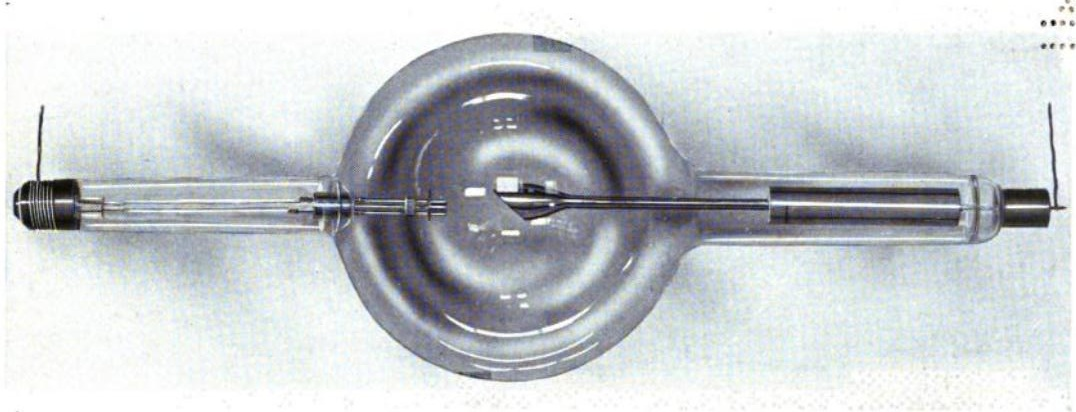
\includegraphics[width=0.6\textwidth]{fotos/dibujotubo.jpg}
            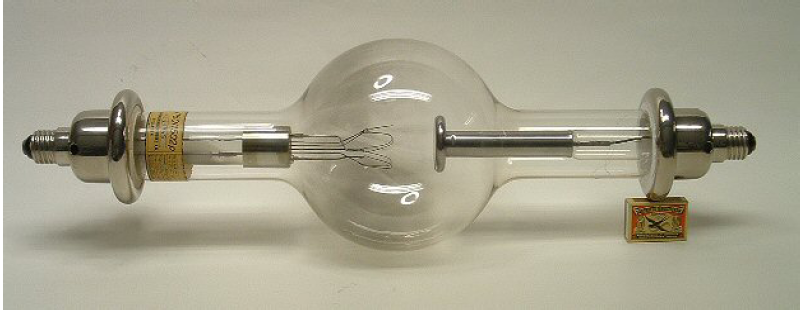
\includegraphics[width=0.6\textwidth]{fotos/foto_tubo.png}
            \caption{Dibuix i fotografia d'un tub de Raigs X}
            \label{fig:raigs X}
        \end{figure}
        
        \clearpage
    \subsection{Efecte Termoiònic}\label{appendix:termoionic}
        L'Efecte Edison o Efecte Termoiònic és d'importància fonamental en l'electromagnetisme. Consisteix en l'augment del flux d'electrons que surten d'un metall o d'un òxid metàl·lic, a causa de les vibracions dels àtoms motivada per l'augment de la temperatura.
        
        \vspace{0.4cm}El fenomen va ser publicat inicialment per \textit{Frederick Guthrie} a Gran Bretanya. \textit{Guthrie} va descobrir que calfant al roig viu una esfera de ferro amb càrrega negativa aquesta perdia la seua càrrega. També va observar que si l'esfera estava carregada positivament el fenomen no apareixia. Altres investigacions al tema foren les realitzades per \textit{William Hittorf} (1869-1883), \textit{Eugen Goldstein} (1885) i \textit{Elster i Geitel} (1882-1889).

        \begin{wrapfigure}{l}{.25\textwidth}
            \vspace{-1.1cm}
            \begin{center}
                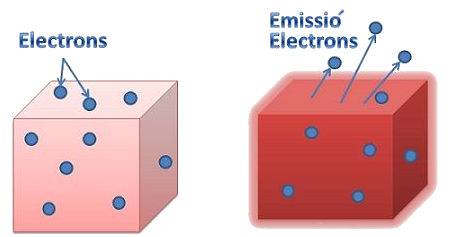
\includegraphics[width=.245\textwidth]{fotos/termoionic.png}
            \end{center}
        \end{wrapfigure}

        \vspace{0.4cm}Històricament, degut a la importància de la seua figura, es va atribuir el seu descobriment a \textit{Thomas Edison}. A 1880, mentre tractava de descobrir perquè es trencaven els filaments y el cristall dels seus llamps incandescents es feia fosc, va redescobrir l'efecte. 
        
        \vspace{0.5cm}\hspace{0cm}Encara que \textit{Edison} no en trobà una aplicació pràctica va patentar el fenomen el 1883 però no l'estudià més. L'efecte unidireccional del corrent es va anomenar Efecte Edison i aquest terme es va utilitzar per referir-se al mateix Efecte Termoiònic. 
        
        \vspace{0.5cm}
        \subsubsection*{Llei de Richardson}

        \begin{wrapfigure}{r}{.25\textwidth}
            \vspace{-0.7cm}
            \begin{center}
                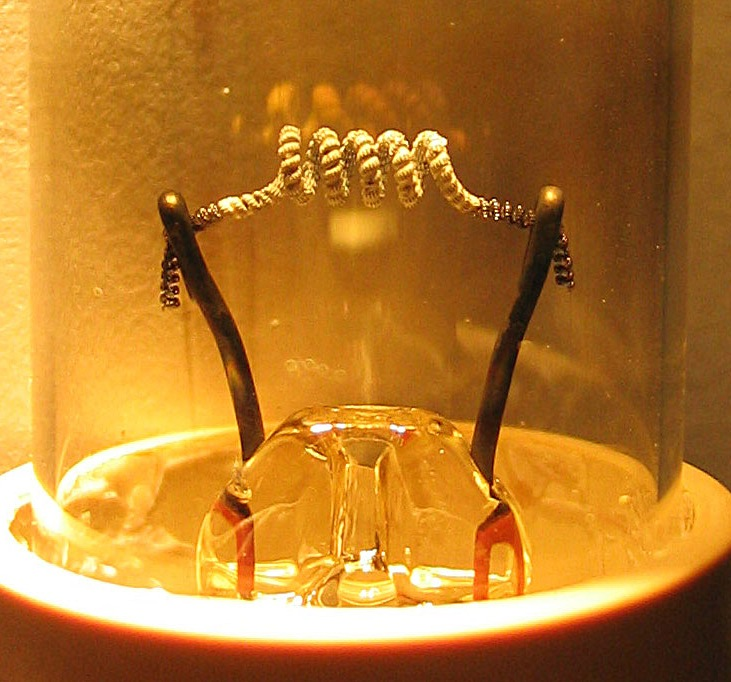
\includegraphics[width=.24\textwidth]{fotos/filament.jpg}
            \end{center}
        \end{wrapfigure}

        \vspace{0.4cm}A 1901, \textit{Owen Willans Richardson} va publicar els resultats dels seus experiments: la corrent procedent d'un filferro pareixia dependre exponencialment de la temperatura del filferro, comportament que era modelat per una formula matemàtica similar a l'Equació d'Arrhenius. La quantitat mínima d'energia necessària perquè un electró surti de la superfície s'anomena funció treball i varia en cada metall. La forma moderna d'aquesta llei (demostrada per Saül Dushman a 1923, i per tant sovint anomenada \textit{equació de Richardson-Dushman}) estableix que la densitat de corrent $J\left[\frac{\si{\ampere}}{\si{\meter}^2}\right]$ està relacionada amb la temperatura T per la equació:
        
        \hspace{0cm}\[J=AT^2e^{\frac{-W}{kT}}\]

        on T es la temperatura en kelvin, W es la funció de treball del metall i k es la constant de Boltzmann i A, la constant coneguda com la constant de Richardson:

        \[A=\frac{4\pi mk^2e}{h^3}=1.20173\times10^6 Am^{-2}K^{-2}\]
        
        on m y -e son la massa y la càrrega de l'electró, y h es la constant de Planck.

    
        \vspace{0.4cm}\textit{Owen Willans Richardson} va rebre un premi Nobel en 1928 per el seu treball en el fenomen termoiònic i especialment per el descobriment de la llei que posteriorment portaria el seu nom.

    \clearpage
    \subsection{Unitats per al camp magnètic}\label{appendix:unitats}
        \vspace{0.2cm}
        A aquest apèndix enumerarem algunes de les diferents unitats utilitzades per a mesurar el camp magnètic i les seues propietats. Podem dividir les unitats que mesuren el comportament dels camps magnètics en funció de si mesuren la intensitat o el flux del mateix.
        \subsubsection*{Unitats de mesura del flux magnètic}
            \begin{itemize}
                \item \textsc{Weber}: Representat simbòlicament per $\si{\weber}$, es la unitat de flux magnètic del Sistema Internacional. Es defineix com al flux magnètic que, a una espira d'una única volta, produiria a la mateixa una fem (força electromotriu) de $1\si{\volt}$ si fora reduït uniformement a 0 en $1\si{\second}$. Rep el seu nom del físic alemany Wilhelm Eduard Weber.
                
                \item \textsc{Maxwell}: Representat simbòlicament per Mx, es una unitat de flux magnètic que s'anomenava \textit{line} abans de 1930, quan va ser adoptat com a unitat del SI fins que a 1935 adoptaren l'actual weber. Un Mx era poc pràctic degut a que era molt petit i solia utilitzar-se la denominació de kilo i megamaxwell ($1$Mx $=10^{-8}\si{\weber}$). Rep el seu nom del físic escocès James Clerk Maxwell.
            \end{itemize}
        \subsubsection*{Unitats de mesura de la intensitat magnètica}
            \begin{itemize}
                \item \textsc{Tesla}: Representat simbòlicament per $\si{\tesla}$, es la unitat de densitat de flux magnètic (o intensitat magnètica) del Sistema Internacional. Es defineix com  la inducció de un camp magnètic que fa una forçat de $1\si{\newton}$ sobre una càrrega de $1\si{\coulomb}$ que es mou a na velocitat de $1\si{\meter}/\si{\second}$ dins del camp, i perpendicularment a les línies d'inducció magnètica. Es a dir, $1\si{\tesla}=1\frac{\si{\newton}\cdot\si{\second}}{\si{\meter}\cdot\si{\coulomb}}$ que en unitats del SI equival a un weber per metre quadrat, $1\si{\tesla}=1\si{\weber}/\si{\meter}^2$. La unitat va ser anunciada la Conferència General de Peses y Mesures a 1960. Rep el seu nom del físic serbi Nikola Tesla.
                \item \textsc{Gauss}: Representat simbòlicament per G, es una unitat de intensitat magnètica. Es defineix utilitzant els Maxwell, $1G = 1\text{Mx}/\si{\cm}^2$. Rep el seu nom del matemàtic i físic alemany Carl Friedrich Gauss.
            \end{itemize}
        \subsubsection*{Equivalències}
            \begin{itemize}
                \item \textsc{Sistema Internacional}
                \[\si{\tesla}=\frac{\si{\volt}\cdot\si{\second}}{\si{\meter}^2} = 
                \frac{\si{\newton}}{\si{\ampere}\cdot\si{\meter}} = 
                \frac{\si{\joule}}{\si{\ampere}\cdot\si{\meter}^2} = 
                \frac{\si{\henry}\cdot\si{\ampere}}{\si{\meter}^2} = 
                \frac{\si{\weber}}{\si{\meter}^2} = 
                \frac{\si{\kilogram}}{\si{\coulomb}\cdot\si{\second}} = 
                \frac{\si{\newton}\cdot\si{\second}}{\si{\coulomb}\cdot\si{\meter}} = 
                \frac{\si{\kilogram}}{\si{\ampere}\cdot\si{\second}^2}
                \]
                \item \textsc{Altres}
                \[\text{G}=\frac{\text{Mx}}{\text{cm}^2}=10^{-4}\si{\tesla}\]
            \end{itemize}
        \clearpage
        
    \subsection{Dades experimentals}\label{appendix:dades}
        Presentem a aquest apèndix les dades experimentals realitzades al laboratori del departament de \textit{Física Aplicada} de la \textit{Universitat d'Alacant}. Recalcar com davant la impossibilitat de mantindre un voltatge constant únic (en la font d'alimentació de les bobines) per a tots els radis que volíem estudiar, vam fer les mesures en voltatges diferents en funció del radi de la trajectòria dels electrons. Tot i això, els intervals equidistants son els mateixos independentment ja que el valor que ens interessa es el de la intensitat que passava per les bobines i no la tensió.
        \begin{table}[h]
            \hspace{-0.3cm}
            \begin{tabular}{
                >{\columncolor[HTML]{ECF4FF}}c cccccc}
                \multicolumn{3}{l}{\cellcolor[HTML]{ECF4FF}Voltatge constant:  6.5 V}                                                                                                                                                                                                 & \multicolumn{1}{l}{} & \multicolumn{3}{l}{\cellcolor[HTML]{ECF4FF}Voltatge constant:  11 V}                                                                                                                                                                                                  \\
                \cellcolor[HTML]{CBCEFB}\textbf{\begin{tabular}[c]{@{}c@{}}$\Delta U$\\  (±1V)\end{tabular}} & \cellcolor[HTML]{CBCEFB}\textbf{\begin{tabular}[c]{@{}c@{}}Intensitat radi \\ 5 cm (±0.01A)\end{tabular}} & \cellcolor[HTML]{CBCEFB}\textbf{\begin{tabular}[c]{@{}c@{}}Intensitat radi \\ 4 cm (±0.01A)\end{tabular}} &                      & \cellcolor[HTML]{CBCEFB}\textbf{\begin{tabular}[c]{@{}c@{}}$\Delta U$\\  (±1V)\end{tabular}} & \cellcolor[HTML]{CBCEFB}\textbf{\begin{tabular}[c]{@{}c@{}}Intensitat radi \\ 3 cm (±0.01A)\end{tabular}} & \cellcolor[HTML]{CBCEFB}\textbf{\begin{tabular}[c]{@{}c@{}}Intensitat radi \\ 2 cm (±0.01A)\end{tabular}} \\
                116                                           & 1.01                                                                                                       & 1.25                                                                                                     &                      & \cellcolor[HTML]{ECF4FF}116                   & 1.73                                                                                                       & 2.54                                                                                                     \\
                \cellcolor[HTML]{DAE8FC}114                   & \cellcolor[HTML]{EFEFEF}0.99                                                                               & \cellcolor[HTML]{EFEFEF}1.25                                                                             &                      & \cellcolor[HTML]{DAE8FC}114                   & \cellcolor[HTML]{EFEFEF}1.72                                                                               & \cellcolor[HTML]{EFEFEF}2.54                                                                             \\
                112                                           & 0.98                                                                                                       & 1.25                                                                                                     &                      & \cellcolor[HTML]{ECF4FF}112                   & 1.67                                                                                                       & 2.48                                                                                                     \\
                \cellcolor[HTML]{DAE8FC}110                   & \cellcolor[HTML]{EFEFEF}0.96                                                                               & \cellcolor[HTML]{EFEFEF}1.19                                                                             &                      & \cellcolor[HTML]{DAE8FC}110                   & \cellcolor[HTML]{EFEFEF}1.66                                                                               & \cellcolor[HTML]{EFEFEF}2.44                                                                             \\
                108                                           & 0.95                                                                                                       & 1.18                                                                                                     &                      & \cellcolor[HTML]{ECF4FF}108                   & 1.63                                                                                                       & 2.44                                                                                                     \\
                \cellcolor[HTML]{DAE8FC}106                   & \cellcolor[HTML]{EFEFEF}0.93                                                                               & \cellcolor[HTML]{EFEFEF}1.16                                                                             &                      & \cellcolor[HTML]{DAE8FC}106                   & \cellcolor[HTML]{EFEFEF}1.62                                                                               & \cellcolor[HTML]{EFEFEF}2.38                                                                             \\
                104                                           & 0.92                                                                                                       & 1.15                                                                                                     &                      & \cellcolor[HTML]{ECF4FF}104                   & 1.61                                                                                                       & 2.38                                                                                                     \\
                \cellcolor[HTML]{DAE8FC}102                   & \cellcolor[HTML]{EFEFEF}0.88                                                                               & \cellcolor[HTML]{EFEFEF}1.15                                                                             &                      & \cellcolor[HTML]{DAE8FC}102                   & \cellcolor[HTML]{EFEFEF}1.57                                                                               & \cellcolor[HTML]{EFEFEF}2.36                                                                             \\
                100                                           & 0.86                                                                                                       & 1.12                                                                                                     &                      & \cellcolor[HTML]{ECF4FF}100                   & 1.54                                                                                                       & 2.34                                                                                                    
            \end{tabular}
            \caption{Dades experimentals}
        \end{table}
    
    \subsection{Càlcul d'errors}\label{appendix:error}
        A aquest apèndix anem a calcular els errors, començant primerament amb els errors instrumentals, que seran: \[\mu\left(r\right)=\frac{0.001}{\sqrt{3}}\si{\meter} \hspace{30mm} \mu\left(V\right)=\frac{5}{\sqrt{12}}\cdot \si{\volt}\hspace{30mm}\mu\left(I\right)=\frac{0.01}{\sqrt{3}}\si{\ampere}\] i amb propagació d'errors arribar a:\[\mu\left(S\ \frac{\Delta U}{r^2}\right)=\sqrt{\left(\frac{-2SV}{r^3}\mu\left(r\right)\right)^2+ \left(\frac{S}{r^2}\mu\left(V\right)\right)^2}\]
    \subsection{Càlcul de les gràfiques i de l'informe}\label{appendix:gràfiques}
        Als següents enllaços es troben el script de \textit{python} que fa les gràfiques que hem vist al llarg de l'informe juntament amb el codi de \textit{LaTeX} que compilat genera este informe.
        \begin{itemize}
            \item \href{https://github.com/vmr48-ua/extras/blob/main/TEC1-MyO1.py}{Enllaç al script de python}
            \item \href{https://www.overleaf.com/read/wfcwdqyrqfct}{Enllaç codi de LaTeX}
        \end{itemize}
        
    \clearpage
\section{Referències}
    \href{https://es.wikipedia.org/wiki/Tubo_de_rayos_cat%C3%B3dicos}{Tubo de rayos catódicos - Wikipedia}\\
    
    \href{https://es.wikipedia.org/wiki/Emisi%C3%B3n_termoi%C3%B3nica}{Efecto Termoiónico - Wikipedia}\\
    
    \href{https://ca.wikipedia.org/wiki/Efecte_Edison}{Efecte Edison - Wikipedia}\\
    
    \href{https://es.wikipedia.org/wiki/Owen_Willans_Richardson}{Owen Willians Richardson - Wikipedia}\\
    
    \href{https://ca.wikipedia.org/wiki/Tub_de_raigs_X}{Tub de raigs X - Wikipedia}\\

    \href{https://es.wikipedia.org/wiki/Rayos_X}{Rayos X - Wikipedia}\\

    \href{https://es.wikipedia.org/wiki/Wilhelm_R%C3%B6ntgen}{Wilhelm Röntgen - Wikipedia}\\
    
    \href{https://www.unav.es/gep/Helmholtz.html}{Helmholtz - UNAV}\\
    
    \href{https://es.wikipedia.org/wiki/Bobina_de_Helmholtz}{Bobina de Helmholtz - Wikipedia}\\
    
    \href{https://es.wikipedia.org/wiki/Weber_(unidad)}{Weber (unidad) - Wikipedia}\\
    
    \href{https://es.wikipedia.org/wiki/Maxwell_(unidad)}{Maxwell (unidad) - Wikipedia}\\
    
    \href{https://es.wikipedia.org/wiki/Tesla_(unidad)}{Tesla (unidad) - Wikipedia}\\
    
    \href{https://es.wikipedia.org/wiki/Gauss_(unidad)}{Gauss (unidad) - Wikipedia}\\
    
    \href{https://es.wikipedia.org/wiki/Relaci%C3%B3n_masa_carga}{Relación masa carga - Wikipedia}\\
    
    \href{http://www.sc.ehu.es/sbweb/fisica/elecmagnet/thomson/Thomson.html}{Medida de la relación carga/masa - sc.ehu.es}\\
    
    \href{https://www.uv.es/inecfis/QPhVL/p3/p3_intro.html}{P3-Relación e/m del electrón - UV}\\
    
    \href{https://www.utm.mx/~labfis/practicas/fisica_moderna/relacion_carga_masa.pdf}{Relación carga/masa del electrón - UTM}\\
    
    \href{https://www.tablesgenerator.com/}{LaTeX tables - tablesgenerator.com}\\
    
    \href{https://es.wikipedia.org/wiki/Permeabilidad_magn%C3%A9tica}{Permebilidad magnética - Wikipedia}\\
    
    \href{https://www.edu.xunta.gal/centros/cafi/aulavirtual/pluginfile.php/40439/mod_imscp/content/2/error_relativo.html#:~:text=El%20error%20relativo%20se%20calcula,absoluto%20entre%20el%20valor%20real.}{Error relativo - edu.xunta.gal}\\
    
    \href{https://www.tochtli.fisica.uson.mx/electro/Constantes_fisicas_fundamentales.htm}{Constantes físicas fundamentales - www.tochtli.fisica.uson.mx}\\
\end{document} 